% !TeX root = main.tex
% header.tex

\documentclass[aspectratio=169, 10pt]{beamer}
\usetheme[progressbar=frametitle]{metropolis}

\usepackage{lmodern}

\usepackage{graphicx}
\usepackage{amssymb}
\usepackage{amsmath}
\usepackage{latexsym}
\usepackage{xcolor}
\usepackage{hyperref}
\usepackage{adjustbox}
\usepackage{mathtools}

\usepackage{multicol}

\usepackage{svg}
\svgpath{{figures/}}

\usepackage{tikz}

% externalize tikz figures to speed up compilation
% \usetikzlibrary{external}
% \tikzexternalize
% \tikzsetexternalprefix{compiled_figures/}
% \tikzexternalize[only named pictures=true]

\usetikzlibrary{arrows, arrows.meta, positioning, shapes.geometric, calc, decorations.pathreplacing, fit}
\usetikzlibrary{backgrounds}
\usetikzlibrary{positioning}
\usetikzlibrary{overlay-beamer-styles}
\usetikzlibrary{angles, quotes}


% 3d tikz
\usepackage{tikz-3dplot}

\definecolor{darkblue}{RGB}{17, 42, 60} % 112A3C
\definecolor{red}{RGB}{175, 49, 39} % AF3127
\definecolor{violet}{RGB}{120, 90, 150} % 785A96
\definecolor{darkviolet}{RGB}{80, 50, 100} % 503264

\definecolor{orange}{RGB}{217, 156, 55} % D99C37
\definecolor{palegreen}{RGB}{197, 184, 104} % C5B868
\definecolor{midorangepalegreen}{RGB}{207, 170, 80} % Approx. CFAB50
\definecolor{green}{RGB}{144, 169, 84} % 90A954
\definecolor{blue}{rgb}{0.38, 0.51, 0.71} %glaucous, 97,130,181,rgb(67, 86, 114)

\definecolor{yellow}{RGB}{250, 199, 100} % FAC764
\definecolor{brokenwhite}{RGB}{218, 192, 166} % DAC0A6
\definecolor{brokengrey}{rgb}{0.77, 0.76, 0.82} % {196,194,209}, C4C2D1

\definecolor{midgreenblue}{RGB}{120, 150, 133} % Between green and blue
\definecolor{midredgreen}{RGB}{160, 109, 62}     % #A06D3E
\definecolor{midredblue}{RGB}{136, 90, 110}      % #885A6E
\definecolor{mixAll}{RGB}{139, 116, 101}         % #8B7465



\colorlet{u}{red!80}
\colorlet{v}{blue!80}
\colorlet{w}{green!80}
\colorlet{A}{midredblue!80}
\colorlet{AA}{mixAll!80}
\makeatletter

% Initialize H matrix for perspective view
\pgfmathsetmacro\H@tpp@aa{1}\pgfmathsetmacro\H@tpp@ab{0}\pgfmathsetmacro\H@tpp@ac{0}%\pgfmathsetmacro\H@tpp@ad{0}
\pgfmathsetmacro\H@tpp@ba{0}\pgfmathsetmacro\H@tpp@bb{1}\pgfmathsetmacro\H@tpp@bc{0}%\pgfmathsetmacro\H@tpp@bd{0}
\pgfmathsetmacro\H@tpp@ca{0}\pgfmathsetmacro\H@tpp@cb{0}\pgfmathsetmacro\H@tpp@cc{1}%\pgfmathsetmacro\H@tpp@cd{0}
\pgfmathsetmacro\H@tpp@da{0}\pgfmathsetmacro\H@tpp@db{0}\pgfmathsetmacro\H@tpp@dc{0}%\pgfmathsetmacro\H@tpp@dd{1}

%Initialize H matrix for main rotation
\pgfmathsetmacro\H@rot@aa{1}\pgfmathsetmacro\H@rot@ab{0}\pgfmathsetmacro\H@rot@ac{0}%\pgfmathsetmacro\H@rot@ad{0}
\pgfmathsetmacro\H@rot@ba{0}\pgfmathsetmacro\H@rot@bb{1}\pgfmathsetmacro\H@rot@bc{0}%\pgfmathsetmacro\H@rot@bd{0}
\pgfmathsetmacro\H@rot@ca{0}\pgfmathsetmacro\H@rot@cb{0}\pgfmathsetmacro\H@rot@cc{1}%\pgfmathsetmacro\H@rot@cd{0}
%\pgfmathsetmacro\H@rot@da{0}\pgfmathsetmacro\H@rot@db{0}\pgfmathsetmacro\H@rot@dc{0}\pgfmathsetmacro\H@rot@dd{1}

\pgfkeys{
    /three point perspective/.cd,
    p/.code args={(#1,#2,#3)}{
            \pgfmathparse{int(round(#1))}
            \ifnum\pgfmathresult=0\else
                \pgfmathsetmacro\H@tpp@ba{#2/#1}
                \pgfmathsetmacro\H@tpp@ca{#3/#1}
                \pgfmathsetmacro\H@tpp@da{ 1/#1}
                \coordinate (vp-p) at (#1,#2,#3);
            \fi
        },
    q/.code args={(#1,#2,#3)}{
            \pgfmathparse{int(round(#2))}
            \ifnum\pgfmathresult=0\else
                \pgfmathsetmacro\H@tpp@ab{#1/#2}
                \pgfmathsetmacro\H@tpp@cb{#3/#2}
                \pgfmathsetmacro\H@tpp@db{ 1/#2}
                \coordinate (vp-q) at (#1,#2,#3);
            \fi
        },
    r/.code args={(#1,#2,#3)}{
            \pgfmathparse{int(round(#3))}
            \ifnum\pgfmathresult=0\else
                \pgfmathsetmacro\H@tpp@ac{#1/#3}
                \pgfmathsetmacro\H@tpp@bc{#2/#3}
                \pgfmathsetmacro\H@tpp@dc{ 1/#3}
                \coordinate (vp-r) at (#1,#2,#3);
            \fi
        },
    coordinate/.code args={#1,#2,#3}{
            \def\tpp@x{#1}
            \def\tpp@y{#2}
            \def\tpp@z{#3}
        },
}

\tikzset{
    view/.code 2 args={
            \pgfmathsetmacro\rot@main@theta{#1}
            \pgfmathsetmacro\rot@main@phi{#2}
            % Row 1
            \pgfmathsetmacro\H@rot@aa{cos(\rot@main@phi)}
            \pgfmathsetmacro\H@rot@ab{sin(\rot@main@phi)}
            \pgfmathsetmacro\H@rot@ac{0}
            % Row 2
            \pgfmathsetmacro\H@rot@ba{-cos(\rot@main@theta)*sin(\rot@main@phi)}
            \pgfmathsetmacro\H@rot@bb{cos(\rot@main@phi)*cos(\rot@main@theta)}
            \pgfmathsetmacro\H@rot@bc{sin(\rot@main@theta)}
            % Row 3
            \pgfmathsetmacro\H@m@ca{sin(\rot@main@phi)*sin(\rot@main@theta)}
            \pgfmathsetmacro\H@m@cb{-cos(\rot@main@phi)*sin(\rot@main@theta)}
            \pgfmathsetmacro\H@m@cc{cos(\rot@main@theta)}
            % Set vector values
            \pgfmathsetmacro\vec@x@x{\H@rot@aa}
            \pgfmathsetmacro\vec@y@x{\H@rot@ab}
            \pgfmathsetmacro\vec@z@x{\H@rot@ac}
            \pgfmathsetmacro\vec@x@y{\H@rot@ba}
            \pgfmathsetmacro\vec@y@y{\H@rot@bb}
            \pgfmathsetmacro\vec@z@y{\H@rot@bc}
            % Set pgf vectors
            \pgfsetxvec{\pgfpoint{\vec@x@x cm}{\vec@x@y cm}}
            \pgfsetyvec{\pgfpoint{\vec@y@x cm}{\vec@y@y cm}}
            \pgfsetzvec{\pgfpoint{\vec@z@x cm}{\vec@z@y cm}}
        },
}

\tikzset{
    perspective/.code={\pgfkeys{/three point perspective/.cd,#1}},
    perspective/.default={p={(15,0,0)},q={(0,15,0)},r={(0,0,50)}},
}

\tikzdeclarecoordinatesystem{three point perspective}{
    \pgfkeys{/three point perspective/.cd,coordinate={#1}}
    \pgfmathsetmacro\temp@p@w{\H@tpp@da*\tpp@x + \H@tpp@db*\tpp@y + \H@tpp@dc*\tpp@z + 1}
    \pgfmathsetmacro\temp@p@x{(\H@tpp@aa*\tpp@x + \H@tpp@ab*\tpp@y + \H@tpp@ac*\tpp@z)/\temp@p@w}
    \pgfmathsetmacro\temp@p@y{(\H@tpp@ba*\tpp@x + \H@tpp@bb*\tpp@y + \H@tpp@bc*\tpp@z)/\temp@p@w}
    \pgfmathsetmacro\temp@p@z{(\H@tpp@ca*\tpp@x + \H@tpp@cb*\tpp@y + \H@tpp@cc*\tpp@z)/\temp@p@w}
    \pgfpointxyz{\temp@p@x}{\temp@p@y}{\temp@p@z}
}
\tikzaliascoordinatesystem{tpp}{three point perspective}

\makeatother

\title{Introduction to Geometric Algebra}
\institute[LIGM]{LIGM, Université Gustave Eiffel}
\author[Harquin]{Enzo Harquin}
\titlegraphic{\includesvg[height=0.15\textheight]{IGM-couleur}}
\date{\today}

\begin{document}


%%%%%%%%%%%%%%%%%%%%%%%%%%%%%%%%%%%%%%%%%%%%%%%%%%%%%%%%%%%%%%%%%%%%%%%%%%%%%%%%%%%%%%%%%%%%%%%%
\begin{frame}
    \titlepage
\end{frame}



\section{Part 1}
\begin{frame}{Formal sum}
    \large
    \begin{center}
        \renewcommand{\arraystretch}{2.0} % more vertical space between rows
        \begin{tabular}{|c|c|}
            \hline
            \textbf{Linear Algebra} & \textbf{Geometric Algebra} \\ \hline
            $\vec{\mathbf{u}} =
                \begin{pmatrix}
                    a \\
                    b \\
                    c \\
                    \vdots
                \end{pmatrix}
                \textcolor{gray}{
                    \begin{pmatrix}
                        \textcolor{red}{e_x}   \\
                        \textcolor{green}{e_y} \\
                        \textcolor{blue}{e_z}  \\
                        \vdots
                    \end{pmatrix}
                }$
                                    &
            $\vec{\mathbf{u}} = a\, \textcolor{red}{e_x} + b\, \textcolor{green}{e_y} + c\, \textcolor{blue}{e_z} + \cdots$
            \\ \hline
        \end{tabular}
    \end{center}
\end{frame}


% \begin{frame}[t]{Inner Product}

%     \visible<1-7>
%     {
%         \begin{center}
%             \Huge $\textcolor{u}{\vec{u}} \cdot \textcolor{v}{\vec{v}}$ \only<4-7>{$= \cos(\textcolor{gray}{\theta}) \|\textcolor{u}{\vec{u}}\| \|\textcolor{v}{\vec{v}}\|$}
%         \end{center}
%     }

%     \begin{columns}[T]
%         \column{0.5\textwidth}

%         \visible<5->
%         {
%             \textbf{Properties:}
%             \begin{itemize}
%                 \item Commutativity
%                 \item Distributivity
%                 \item Linearity
%             \end{itemize}
%         }

%         \vspace{2em}

%         \visible<6-7>
%         {
%             \begin{alertblock}{Limitations}
%                 Not enough information about the vectors
%             \end{alertblock}
%         }

%         \column{0.5\textwidth}
%         \begin{minipage}[c][0.6\textheight][c]{\linewidth} % [c] vertical alignment, [\textheight] height, [c] content alignment
%             \centering
%             \begin{tikzpicture}
%                 \coordinate (O) at (0,0);

%                 \def\xa{2.5}
%                 \def\ya{2.5}
%                 \coordinate (a) at (\xa,\ya);

%                 \def\xb{4}
%                 \def\yb{0}
%                 \coordinate (b) at (\xb,\yb);

%                 \visible<2-6>
%                 {
%                     \draw[ultra thick, u, ->, >=Triangle] (O) -- (a);
%                     \draw[ultra thick, v, ->, >=Triangle] (O) -- (b);
%                 }

%                 \visible<3-6>
%                 {
%                     \draw[ultra thick, gray, dotted, overlay] (\xa,0) -- (\xa, \ya);
%                 }

%                 \visible<3>
%                 {
%                     \draw[decorate,gray, ultra thick,decoration={brace,amplitude=10pt,mirror}] (O) -- (\xa, 0) node[midway,below,yshift=-10pt] {Proj}; % Label for the magnitude
%                 }

%                 \visible<4-6>
%                 {
%                     \draw pic[
%                             ultra thick,
%                             gray,
%                             draw=gray,
%                             angle radius=1cm,
%                             angle eccentricity=1.2,
%                             "$\theta$"
%                         ] {angle=b--O--a};

%                     \draw[decorate,gray, ultra thick,decoration={brace,amplitude=10pt,mirror}] (O) -- (\xa, 0) node[midway,below,yshift=-10pt] {$\cos(\textcolor{gray}{\theta}) \|\textcolor{u}{\vec{u}}\| \|\textcolor{v}{\vec{v}}\|$}; % Label for the magnitude
%                 }

%                 \visible<7>
%                 {
%                     \def\xa{2.5}
%                     \def\ya{-2.5}
%                     \coordinate (a) at (\xa,\ya);

%                     \def\xb{4}
%                     \def\yb{0}
%                     \coordinate (b) at (\xb,\yb);

%                     \draw[ultra thick, u, ->, >=Triangle] (O) -- (a);
%                     \draw[ultra thick, v, ->, >=Triangle] (O) -- (b);

%                     \draw[ultra thick, gray, dotted, overlay] (\xa,0) -- (\xa, \ya);

%                     \draw pic[
%                             ultra thick,
%                             gray,
%                             draw=gray,
%                             angle radius=1cm,
%                             angle eccentricity=1.2,
%                             "$\theta$"
%                         ] {angle=a--O--b};

%                     \draw[decorate,gray, ultra thick,decoration={brace,amplitude=10pt}] (O) -- (\xa, 0) node[midway,below,yshift=30pt] {$\cos(\textcolor{gray}{\theta}) \|\textcolor{u}{\vec{u}}\| \|\textcolor{v}{\vec{v}}\|$}; % Label for the magnitude
%                 }
%             \end{tikzpicture}
%         \end{minipage}
%     \end{columns}
% \end{frame}


% \begin{frame}[t]{(Not the) Cross Product}
%     \begin{center}
%         \Huge $\textcolor{u}{\vec{u}} \times \textcolor{v}{\vec{v}}$ \only<2>{$ = \|\textcolor{u}{\vec{u}}\| \|\textcolor{v}{\vec{v}}\| \sin(\textcolor{gray}{\theta}) \hat{n}$}
%     \end{center}

%     \vspace{3em}

%     \begin{columns}[T]
%         \column{0.5\textwidth}
%         \visible<3>
%         {
%             \begin{alertblock}{Problem}
%                 Only works in 3D \ldots
%             \end{alertblock}
%         }

%     \end{columns}

% \end{frame}

% \begin{frame}[t]{New Operator}
%     \centering
%     \Huge
%     An operator that
%     \only<1>{\dots}
%     \only<2>{\\\textbf{increases the dimension}?}

%     \vspace{2em}

%     \only<2>{
%         \Large
%         \begin{minipage}{0.8\textwidth}
%             The \textbf{inner product} between two vectors gives a scalar: it \textbf{contracts} dimensions.\\[1em]
%             But what if we want to \textbf{expand} dimensionality?\\[1em]
%         \end{minipage}
%     }
% \end{frame}


\begin{frame}[t]{Bivectors and Outer Product}

    \begin{center}
        \only<1-3>{\Huge $\textcolor{u}{\vec{u}} \wedge \textcolor{v}{\vec{v}}$ \only<3-4>{$=\textcolor{A}{\vec{A}}$}}
        % \only<4-5>{\Huge $\textcolor{v}{\vec{v}} \wedge \textcolor{u}{\vec{u}}$ \only<5>{$=\textcolor{A}{-\vec{A}}$}}
        \only<4>{\Huge $\textcolor{u}{\vec{u}} \wedge \textcolor{v}{\vec{v}}=-\textcolor{v}{\vec{v}} \wedge \textcolor{u}{\vec{u}}$}
        \only<5>{\Huge $\textcolor{A}{\vec{A}}$}
        \only<6-7>{\Huge $\|\textcolor{A}{\vec{A}}\|$ \only<7>{$=\sin(\textcolor{gray}{\theta}) \|\textcolor{u}{\vec{u}}\| \|\textcolor{v}{\vec{v}}\|$}}
        \only<8>{\Huge $\|\textcolor{A}{\vec{A}}\| = 0$}
    \end{center}

    \begin{minipage}[c][0.6\textheight][c]{\linewidth}
        \centering
        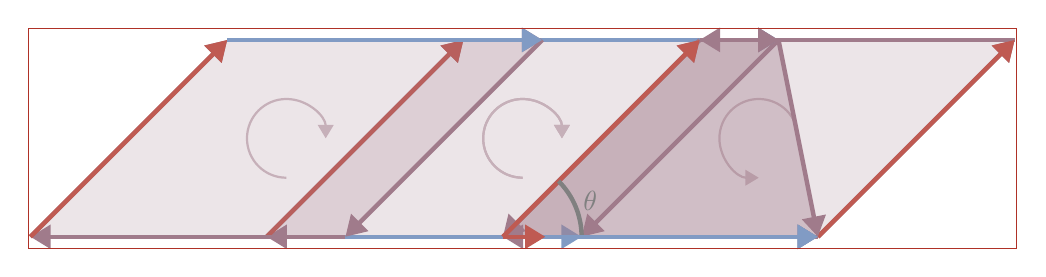
\begin{tikzpicture}
            \coordinate (O) at (0,0);

            \def\xa{2.5}
            \def\ya{2.5}
            \coordinate (a) at (\xa,\ya);

            \def\xb{4}
            \def\yb{0}
            \coordinate (b) at (\xb,\yb);

            \visible<3>
            {
                \draw[ultra thick, A, ->, >=Triangle] ({\xa+\xb},{\ya}) -- (b);
                \draw[ultra thick, A, ->, >=Triangle] (a) -- ({\xa+\xb},{\ya});
                \draw[ultra thick, A, ->, >=Triangle] (b) -- (O);
                \draw[ultra thick, A, ->, >=Triangle] (O) -- (a);

                \draw[draw=none, fill=A, opacity=0.2] ({\xa+\xb},{\ya}) -- (b) -- (O) -- (a) -- cycle;
                % \node[A] at (3,1.25) {$\vec{A}$};
                \draw[A!60, thick,<-,>=Triangle] (3.75,1.25) arc[radius=0.5cm,start angle=0,delta angle=270];
                % point on the center of the parallelogram
            }

            \visible<1-3>
            {
                \draw[ultra thick, u, ->, >=Triangle] (O) -- (a);
            }

            \visible<1>
            {
                \draw[ultra thick, v, ->, >=Triangle] (O) -- (b);
            }

            \visible<2-3>
            {
                \draw[ultra thick, v, ->, >=Triangle] (a) -- ({\xa+\xb},{\ya});
            }


            % \visible<5>
            % {
            %     \draw[ultra thick, A, <-, >=Triangle] ({\xa+\xb},{\ya}) -- (b);
            %     \draw[ultra thick, A, <-, >=Triangle] (a) -- ({\xa+\xb},{\ya});
            %     \draw[ultra thick, A, <-, >=Triangle] (b) -- (O);
            %     \draw[ultra thick, A, <-, >=Triangle] (O) -- (a);

            %     \draw[draw=none, fill=A, opacity=0.2] ({\xa+\xb},{\ya}) -- (b) -- (O) -- (a) -- cycle;
            %     % \node[A] at (3,1.25) {$\vec{A}$};
            %     \draw[A!60, thick,->,>=Triangle] (3.75,1.25) arc[radius=0.5cm,start angle=0,delta angle=270];
            %     % point on the center of the parallelogram
            % }

            % \visible<4-5>
            % {
            %     \draw[ultra thick, v, ->, >=Triangle] (O) -- (b);
            %     \draw[ultra thick, u, ->, >=Triangle] (b) -- ({\xa+\xb},{\ya});
            % }

            \only<4>
            {
                \begin{scope}[shift={(-3,0)}]
                    \coordinate (O) at (0,0);

                    \def\xa{2.5}
                    \def\ya{2.5}
                    \coordinate (a) at (\xa,\ya);

                    \def\xb{4}
                    \def\yb{0}
                    \coordinate (b) at (\xb,\yb);

                    \draw[ultra thick, A, ->, >=Triangle] ({\xa+\xb},{\ya}) -- (b);
                    \draw[ultra thick, A, ->, >=Triangle] (a) -- ({\xa+\xb},{\ya});
                    \draw[ultra thick, A, ->, >=Triangle] (b) -- (O);
                    \draw[ultra thick, A, ->, >=Triangle] (O) -- (a);

                    \draw[draw=none, fill=A, opacity=0.2] ({\xa+\xb},{\ya}) -- (b) -- (O) -- (a) -- cycle;
                    % \node[A] at (3,1.25) {$\vec{A}$};
                    \draw[A!60, thick,<-,>=Triangle] (3.75,1.25) arc[radius=0.5cm,start angle=0,delta angle=270];
                    % point on the center of the parallelogram
                    \draw[ultra thick, u, ->, >=Triangle] (O) -- (a);
                    \draw[ultra thick, v, ->, >=Triangle] (a) -- ({\xa+\xb},{\ya});
                \end{scope}

                \begin{scope}[shift={(3,0)}]
                    \coordinate (O) at (0,0);

                    \def\xa{2.5}
                    \def\ya{2.5}
                    \coordinate (a) at (\xa,\ya);

                    \def\xb{4}
                    \def\yb{0}
                    \coordinate (b) at (\xb,\yb);

                    \draw[ultra thick, A, <-, >=Triangle] ({\xa+\xb},{\ya}) -- (b);
                    \draw[ultra thick, A, <-, >=Triangle] (a) -- ({\xa+\xb},{\ya});
                    \draw[ultra thick, A, <-, >=Triangle] (b) -- (O);
                    \draw[ultra thick, A, <-, >=Triangle] (O) -- (a);

                    \draw[draw=none, fill=A, opacity=0.2] ({\xa+\xb},{\ya}) -- (b) -- (O) -- (a) -- cycle;
                    % \node[A] at (3,1.25) {$\vec{A}$};
                    \draw[A!60, thick,->,>=Triangle] (3.75,1.25) arc[radius=0.5cm,start angle=0,delta angle=270];
                    % point on the center of the parallelogram

                    \draw[ultra thick, v, ->, >=Triangle] (O) -- (b);
                    \draw[ultra thick, u, ->, >=Triangle] (b) -- ({\xa+\xb},{\ya});
                \end{scope}

            }

            \visible<5>
            {
                \draw[ultra thick, A, ->, >=Triangle] ({\xa+\xb},{\ya}) -- (b);
                \draw[ultra thick, A, ->, >=Triangle] (a) -- ({\xa+\xb},{\ya});
                \draw[ultra thick, A, ->, >=Triangle] (b) -- (O);
                \draw[ultra thick, A, ->, >=Triangle] (O) -- (a);

                \draw[draw=none, fill=A, opacity=0.2] ({\xa+\xb},{\ya}) -- (b) -- (O) -- (a) -- cycle;
                % \node[A] at (3,1.25) {$\vec{A}$};
                \draw[A!60, thick,<-,>=Triangle] (3.75,1.25) arc[radius=0.5cm,start angle=0,delta angle=270];
                % point on the center of the parallelogram
            }

            \visible<6-7>
            {
                \draw[draw=none, fill=A, opacity=0.2] ({\xa+\xb},{\ya}) -- (b) -- (O) -- (a) -- cycle;
            }

            \visible<7>
            {
                \draw[ultra thick, u, ->, >=Triangle] (O) -- (a);
                \draw[ultra thick, v, ->, >=Triangle] (O) -- (b);

                \draw pic[
                        ultra thick,
                        gray,
                        draw=gray,
                        angle radius=1cm,
                        angle eccentricity=1.2,
                        "$\theta$"
                    ] {angle=b--O--a};
            }

            \visible<8>
            {
                \draw[ultra thick, v, ->, >=Triangle] (O) -- (b);
                \draw[ultra thick, u, ->, >=Triangle] (O) -- ({3.54},{0});
            }

            \draw[red] (current bounding box.south west) rectangle (current bounding box.north east);

        \end{tikzpicture}

    \end{minipage}

    \centering
    \huge
    \only<4>{Anti-Commutativity!}
    \only<8>{Contract parallel dimensions!}


\end{frame}



\begin{frame}[t]{Bivectors and Outer Product}

    \begin{center}
        \only<1-2>{\Huge $\textcolor{u}{\vec{u}} \wedge \textcolor{v}{\vec{v}} =\textcolor{A}{\vec{A}}$}
    \end{center}

    \begin{columns}

        \column{0.5\textwidth}
        \only<1-2>
        {
            \begin{tabular}{rcl}
                $\lambda \wedge \textcolor{u}{\vec{u}}$                                                & $=$ & $\lambda\,\textcolor{u}{\vec{u}}$                                                                                 \\
                $(\textcolor{u}{\vec{u}} \wedge \textcolor{v}{\vec{v}}) \wedge \textcolor{w}{\vec{w}}$ & $=$ & $\textcolor{u}{\vec{u}} \wedge (\textcolor{v}{\vec{v}} \wedge \textcolor{w}{\vec{w}})$                            \\
                $\textcolor{u}{\vec{u}} \wedge (\textcolor{v}{\vec{v}} + \textcolor{w}{\vec{w}})$      & $=$ & $(\textcolor{u}{\vec{u}} \wedge \textcolor{v}{\vec{v}}) + (\textcolor{u}{\vec{u}} \wedge \textcolor{w}{\vec{w}})$ \\
                $\textcolor{u}{\vec{u}} \wedge (\lambda \textcolor{v}{\vec{v}})$                       & $=$ & $\lambda\,(\textcolor{u}{\vec{u}} \wedge \textcolor{v}{\vec{v}})$                                                 \\
                \\
                $\textcolor{u}{\vec{u}} \wedge \textcolor{v}{\vec{v}}$                                 & $=$ & $-\textcolor{v}{\vec{v}} \wedge \textcolor{u}{\vec{u}}$                                                           \\
                $\textcolor{u}{\vec{u}} \wedge \lambda \textcolor{u}{\vec{u}}$                         & $=$ & $0$                                                                                                               \\
            \end{tabular}
        }

        \vspace{2em}

        \only<2>
        {
            \begin{alertblock}{Limitations (again)}
                Not enough information about the vectors
            \end{alertblock}
        }


        \column{0.5\textwidth}
        \begin{minipage}[c][0.6\textheight][c]{\linewidth} % [c] vertical alignment, [\textheight] height, [c] content alignment
            \centering
            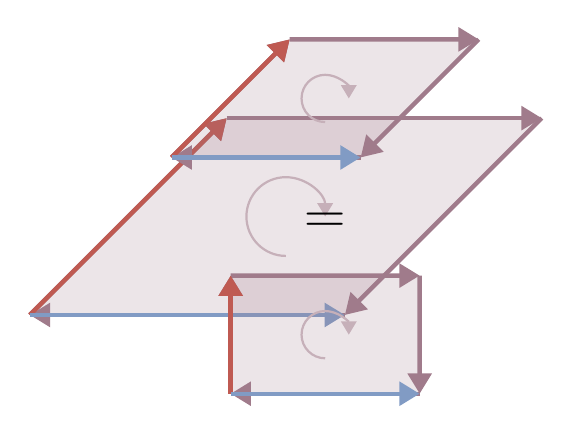
\begin{tikzpicture}

                \visible<1>
                {
                    \begin{scope}[shift={(0,-2)}]
                        \coordinate (O) at (0,0);

                        \def\xa{2.5}
                        \def\ya{2.5}
                        \coordinate (a) at (\xa,\ya);

                        \def\xb{4}
                        \def\yb{0}
                        \coordinate (b) at (\xb,\yb);

                        \draw[ultra thick, A, ->, >=Triangle] ({\xa+\xb},{\ya}) -- (b);
                        \draw[ultra thick, A, ->, >=Triangle] (a) -- ({\xa+\xb},{\ya});
                        \draw[ultra thick, A, ->, >=Triangle] (b) -- (O);
                        \draw[ultra thick, A, ->, >=Triangle] (O) -- (a);

                        \draw[draw=none, fill=A, opacity=0.2] ({\xa+\xb},{\ya}) -- (b) -- (O) -- (a) -- cycle;
                        % \node[A] at (3,1.25) {$\vec{A}$};
                        \draw[A!60, thick,<-,>=Triangle] (3.75,1.25) arc[radius=0.5cm,start angle=0,delta angle=270];
                        % point on the center of the parallelogram

                        \draw[ultra thick, u, ->, >=Triangle] (O) -- (a);
                        \draw[ultra thick, v, ->, >=Triangle] (O) -- (b);
                    \end{scope}
                }


                \visible<2>
                {
                    \begin{scope}[scale=0.6, shift={(3,0)}]
                        \coordinate (O) at (0,0);

                        \def\xa{2.5}
                        \def\ya{2.5}
                        \coordinate (a) at (\xa,\ya);

                        \def\xb{4}
                        \def\yb{0}
                        \coordinate (b) at (\xb,\yb);

                        \draw[ultra thick, A, ->, >=Triangle] ({\xa+\xb},{\ya}) -- (b);
                        \draw[ultra thick, A, ->, >=Triangle] (a) -- ({\xa+\xb},{\ya});
                        \draw[ultra thick, A, ->, >=Triangle] (b) -- (O);
                        \draw[ultra thick, A, ->, >=Triangle] (O) -- (a);

                        \draw[draw=none, fill=A, opacity=0.2] ({\xa+\xb},{\ya}) -- (b) -- (O) -- (a) -- cycle;
                        % \node[A] at (3,1.25) {$\vec{A}$};
                        \draw[A!60, thick,<-,>=Triangle] (3.75,1.25) arc[radius=0.5cm,start angle=0,delta angle=270];
                        % point on the center of the parallelogram

                        \draw[ultra thick, u, ->, >=Triangle] (O) -- (a);
                        \draw[ultra thick, v, ->, >=Triangle] (O) -- (b);

                        \node at (3.25,-1.4) {\huge$=$};

                        \begin{scope}[shift={(1.25,-5)}]
                            \coordinate (O) at (0,0);

                            \def\xa{0}
                            \def\ya{2.5}
                            \coordinate (a) at (\xa,\ya);

                            \def\xb{4}
                            \def\yb{0}
                            \coordinate (b) at (\xb,\yb);

                            \draw[ultra thick, A, ->, >=Triangle] ({\xa+\xb},{\ya}) -- (b);
                            \draw[ultra thick, A, ->, >=Triangle] (a) -- ({\xa+\xb},{\ya});
                            \draw[ultra thick, A, ->, >=Triangle] (b) -- (O);
                            \draw[ultra thick, A, ->, >=Triangle] (O) -- (a);

                            \draw[draw=none, fill=A, opacity=0.2] ({\xa+\xb},{\ya}) -- (b) -- (O) -- (a) -- cycle;
                            % \node[A] at (3,1.25) {$\vec{A}$};
                            \draw[A!60, thick,<-,>=Triangle] (2.5,1.25) arc[radius=0.5cm,start angle=0,delta angle=270];
                            % point on the center of the parallelogram

                            \draw[ultra thick, u, ->, >=Triangle] (O) -- (a);
                            \draw[ultra thick, v, ->, >=Triangle] (O) -- (b);

                        \end{scope}
                    \end{scope}
                }
            \end{tikzpicture}
        \end{minipage}

    \end{columns}

\end{frame}


\begin{frame}{Bivector in 2D}
    \Large
    \[
        \textcolor{u}{\vec{u}} = a_1 \textcolor{red}{\mathbf{e}_x} + b_1 \textcolor{green}{\mathbf{e}_y}
        \qquad
        \textcolor{v}{\vec{v}} = a_2 \textcolor{red}{\mathbf{e}_x} + b_2 \textcolor{green}{\mathbf{e}_y}
    \]

    \begin{align*}
        \textcolor{u}{\vec{u}} \wedge \textcolor{v}{\vec{v}}
         & = (a_1 \textcolor{red}{\mathbf{e}_x} + b_1 \textcolor{green}{\mathbf{e}_y}) \wedge (a_2 \textcolor{red}{\mathbf{e}_x} + b_2 \textcolor{green}{\mathbf{e}_y}) \\
         & = a_1 a_2 (\textcolor{red}{\mathbf{e}_x} \wedge \textcolor{red}{\mathbf{e}_x})
        + a_1 b_2 (\textcolor{red}{\mathbf{e}_x} \wedge \textcolor{green}{\mathbf{e}_y})                                                                                \\
         & \quad + b_1 a_2 (\textcolor{green}{\mathbf{e}_y} \wedge \textcolor{red}{\mathbf{e}_x})
        + b_1 b_2 (\textcolor{green}{\mathbf{e}_y} \wedge \textcolor{green}{\mathbf{e}_y})                                                                              \\
         & = (a_1 b_2 - b_1 a_2)(\textcolor{red}{\mathbf{e}_x} \wedge \textcolor{green}{\mathbf{e}_y})                                                                  \\
         & = (a_1 b_2 - b_1 a_2) \textcolor{midredgreen}{\mathbf{e}_{xy}}
    \end{align*}
\end{frame}


\begin{frame}{Bivector in 3D}
    \Large
    \[
        \textcolor{u}{\vec{u}} = a_1 \textcolor{red}{\mathbf{e}_x} + b_1 \textcolor{green}{\mathbf{e}_y} + c_1 \textcolor{blue}{\mathbf{e}_z}
        \quad\quad
        \textcolor{v}{\vec{v}} = a_2 \textcolor{red}{\mathbf{e}_x} + b_2 \textcolor{green}{\mathbf{e}_y} + c_2 \textcolor{blue}{\mathbf{e}_z}
    \]

    \vspace{0.5em}

    \begin{align*}
        \textcolor{u}{\vec{u}} \wedge \textcolor{v}{\vec{v}} & =
        (a_1 b_2 - b_1 a_2)\, \textcolor{midredgreen}{\mathbf{e}_{xy}}
        + (c_1 a_2 - a_1 c_2)\, \textcolor{midredblue}{\mathbf{e}_{zx}}
        + (b_1 c_2 - c_1 b_2)\, \textcolor{midgreenblue}{\mathbf{e}_{yz}}
        \\
        \textcolor{u}{\vec{u}} \times \textcolor{v}{\vec{v}} & =
        (a_1 b_2 - b_1 a_2)\, \textcolor{blue}{\mathbf{e}_z}
        + (c_1 a_2 - a_1 c_2)\, \textcolor{green}{\mathbf{e}_y}
        + (b_1 c_2 - c_1 b_2)\, \textcolor{red}{\mathbf{e}_x}
    \end{align*}

    \vspace{0.5em}

    \textbf{Note}: looks like the cross product of \(\mathbb{R}^3\) but:
    \begin{itemize}
        \item is actually defined in any dimension
        \item is associative: \((\textcolor{u}{\vec{u}} \wedge \textcolor{v}{\vec{v}}) \wedge \textcolor{w}{\vec{w}} = \textcolor{u}{\vec{u}} \wedge (\textcolor{v}{\vec{v}} \wedge \textcolor{w}{\vec{w}})\)
    \end{itemize}
\end{frame}




\begin{frame}[t]{Trivectors}

  \begin{center}
    \Huge
    $\textcolor{u}{\vec{u}} \wedge \textcolor{v}{\vec{v}} \wedge \textcolor{w}{\vec{w}} =\textcolor{AA}{A}$
  \end{center}

  \setlength{\columnsep}{20pt}
  \begin{columns}[T]
    \column{0.5\textwidth}

    \textbf{Properties}:
    \begin{itemize}
      \item Magnitude (Volume)
      \item Orientation
    \end{itemize}

    \textbf{Operations:}
    \begin{itemize}
      \item Addition
      \item Multiplication by a scalar
      \item \ldots
    \end{itemize}

    \column{0.5\textwidth}
    \begin{minipage}[c][0.5\textheight][c]{\linewidth} % [c] vertical alignment, [\textheight] height, [c] content alignment
      \centering
      \begin{tikzpicture}[remember picture]
        \useasboundingbox (-3,-3) rectangle (3,3);

        \begin{scope}[
            scale=2,
            view={60}{135},
            perspective={
                p={(-10,0,0)},
                q={(0,-10,0)},
                r={(0,0,-60)}
              },
            bullet/.style={circle,fill,inner sep=1pt},font=\sffamily,
            cube/.style={very thick,black},
            grid/.style={opacity=0.1, very thin,gray},
            vec/.style={->, >=triangle 45, ultra thick, yellow},
            axis/.style={dotted, thick},
            bivector/.style={draw=none,fill=yellow, opacity=0.2}]

          % Draw a grid in the x-y plane
          \foreach \x in {-0.5,0,...,1.5}
          \foreach \y in {-0.5,0,...,1.5}
            {
              \draw[opacity=0.1, very thin,gray] (tpp cs:\x,-0.5,0) -- (tpp cs:\x,1.5,0);
              \draw[opacity=0.1, very thin,gray] (tpp cs:-0.5,\y,0) -- (tpp cs:1.5,\y,0);
            }

          % Draw the axes
          \draw[axis] (tpp cs:-0.5,0,0) -- (tpp cs:1.5,0,0);
          \draw[axis] (tpp cs:0,-0.5,0) -- (tpp cs:0,1.5,0);
          \draw[axis] (tpp cs:0,0,0) -- (tpp cs:0,0,1.5);

          \coordinate (A) at (tpp cs:0,0,0);
          \coordinate (B) at (tpp cs:1,0,0);
          \coordinate (C) at (tpp cs:1,1,0);
          \coordinate (D) at (tpp cs:0,1,0);
          \coordinate (E) at (tpp cs:0,0,1);
          \coordinate (F) at (tpp cs:1,0,1);
          \coordinate (G) at (tpp cs:1,1,1);
          \coordinate (H) at (tpp cs:0,1,1);

          % Draw edges of the cube
          \draw[vec, opacity=0.5, u, >=latex] (A) -- (B);
          \draw[vec, opacity=0.5, v, >=latex] (B) -- (C);
          \draw[vec, opacity=0.5, AA, >=latex] (C) -- (D);
          \draw[vec, opacity=0.5, AA, >=latex] (D) -- (A);

          \draw[vec, opacity=0.5, AA, >=latex] (E) -- (F);
          \draw[vec, opacity=0.5, AA, >=latex] (F) -- (G);
          \draw[vec, opacity=0.5, AA, >=latex] (G) -- (H);
          \draw[vec, opacity=0.5, AA, >=latex] (H) -- (E);

          \draw[vec, opacity=0.5, AA, >=latex] (A) -- (E);
          \draw[vec, opacity=0.5, AA, >=latex] (B) -- (F);
          \draw[vec, opacity=0.5, w, >=latex] (C) -- (G);
          \draw[vec, opacity=0.5, AA, >=latex] (D) -- (H);

          % draw face of the cube
          \draw[bivector, AA] (B) -- (F) -- (G) -- (C) -- cycle;
          \draw[bivector, AA] (E) -- (F) -- (G) -- (H) -- cycle;
          \draw[bivector, AA] (C) -- (D) -- (H) -- (G) -- cycle;

        \end{scope}
        %\draw[red] (current bounding box.south west) rectangle (current bounding box.north east);
      \end{tikzpicture}
    \end{minipage}

  \end{columns}

\end{frame}




\begin{frame}{$k$-vectors and subspaces}
    \textbf{Set of vector spaces in 3D:}

    \vspace{1em}

    \[
        \left\{
        \underbrace{\mathbf{1}}_{\text{scalar}},\quad
        \underbrace{
            \textcolor{red}{\mathbf{e}_x},\
            \textcolor{green}{\mathbf{e}_y},\
            \textcolor{blue}{\mathbf{e}_z}
        }_{\text{vector space}},\quad
        \underbrace{
            \textcolor{midredgreen}{\mathbf{e}_{xy}},\
            \textcolor{midredblue}{\mathbf{e}_{zx}},\
            \textcolor{midgreenblue}{\mathbf{e}_{yz}}
        }_{\text{bivector space}},\quad
        \underbrace{
            \textcolor{mixAll}{\mathbf{e}_{xyz}}
        }_{\text{trivector space}}
        \right\}
    \]

    \vspace{1em}

    \textbf{Pseudo-scalar: }
    \(
    \textcolor{mixAll}{\mathbf{I}} =
    \textcolor{red}{\mathbf{e}_x} \wedge
    \textcolor{green}{\mathbf{e}_y} \wedge
    \textcolor{blue}{\mathbf{e}_z} =
    \textcolor{mixAll}{\mathbf{e}_{xyz}}
    \)
\end{frame}

\section{Part 2}
\begin{frame}{Metric $\mathbb{R}_{3,0,1}$}
    \textbf{3D Projective geometric algebra:} \quad $\mathbb{R}_{3,0,1}$

    \begin{columns}
        \column{0.5\textwidth}
        \begin{center}
            \begin{tabular}{c|cccc}
                                                  & $\textcolor{red}{\mathbf{e}_x}$ & $\textcolor{green}{\mathbf{e}_y}$ & $\textcolor{blue}{\mathbf{e}_z}$ & $\textcolor{gray}{\mathbf{e}_0}$ \\ \hline
                $\textcolor{red}{\mathbf{e}_x}$   & 1                               & \textcolor{gray}{0}               & \textcolor{gray}{0}              & \textcolor{gray}{0}              \\
                $\textcolor{green}{\mathbf{e}_y}$ & \textcolor{gray}{0}             & 1                                 & \textcolor{gray}{0}              & \textcolor{gray}{0}              \\
                $\textcolor{blue}{\mathbf{e}_z}$  & \textcolor{gray}{0}             & \textcolor{gray}{0}               & 1                                & \textcolor{gray}{0}              \\
                $\textcolor{gray}{\mathbf{e}_0}$  & \textcolor{gray}{0}             & \textcolor{gray}{0}               & \textcolor{gray}{0}              & 0                                \\
            \end{tabular}
        \end{center}
        \column{0.5\textwidth}

        \begin{align*}
            \mathbf{p}       & = x\,\textcolor{red}{\mathbf{e}_x} + y\,\textcolor{green}{\mathbf{e}_y} + z\,\textcolor{blue}{\mathbf{e}_z} + w\,\textcolor{gray}{\mathbf{e}_0} \\
            \vec{\mathbf{u}} & = a\,\textcolor{red}{\mathbf{e}_x} + b\,\textcolor{green}{\mathbf{e}_y} + c\,\textcolor{blue}{\mathbf{e}_z}
        \end{align*}

    \end{columns}

\end{frame}




\begin{frame}[t]{Line from points and vectors}

    $$
        \mathbf{p} =
        x\textcolor{red}{\mathbf{e}_x} +
        y\textcolor{green}{\mathbf{e}_y} +
        z\textcolor{blue}{\mathbf{e}_z} +
        w\textcolor{gray}{\mathbf{e}_0}
        \qquad
        \vec{\mathbf{u}} =
        a\textcolor{red}{\mathbf{e}_x} +
        b\textcolor{green}{\mathbf{e}_y} +
        c\textcolor{blue}{\mathbf{e}_z}
    $$


    \vspace{0.5em}

    % Two-column layout
    \begin{columns}
        \column{0.5\textwidth}
        \centering
        \visible<2->{$\mathbf{L} = $} $\mathbf{p}_1 \wedge \only<1-2>{\mathbf{p}_2} \only<3->{\textcolor{u}{\vec{\mathbf{u}}}}$


        \column{0.5\textwidth}
        \begin{center}
            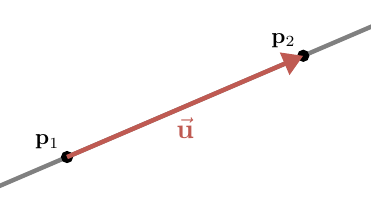
\begin{tikzpicture}
                \useasboundingbox (-2,-1) rectangle (2,1);

                \filldraw (-1.5, -0.643) circle (2pt) node[above left, scale=0.8] {$\mathbf{p}_1$};

                \visible<1-2>{\filldraw (1.5, 0.643) circle (2pt) node[above left, scale=0.8] {$\mathbf{p}_2$};}
                \visible<3->{\draw[u,>=Triangle,->, ultra thick] (-1.5, -0.643) -- (1.5, 0.643) node[midway, below] {$\vec{\mathbf{u}}$};}
                \only<2->{
                    \begin{scope}[on background layer]
                        \def\xa{3.5}
                        \def\ya{1.5}
                        \def\scaleFactor{5}
                        \draw[ultra thick, gray, overlay] ({-\scaleFactor*\xa}, {- \scaleFactor*\ya}) -- ({\scaleFactor*\xa}, {\scaleFactor*\ya});
                    \end{scope}
                }


                %\draw[red] (current bounding box.south west) rectangle (current bounding box.north east);
            \end{tikzpicture}
        \end{center}
    \end{columns}

    \vspace{3em}

    \begin{center}
        \visible<4->
        {
            $$
                \mathbf{p} \in \mathbf{L}
                \qquad \Leftrightarrow \qquad
                \mathbf{L} \wedge \mathbf{p} = 0
            $$
        }
        \visible<5->{
            \ldots corresponds to Plücker lines!
        }
    \end{center}
\end{frame}



\begin{frame}[t]{Plane from points and vectors}

    $$
        \mathbf{p} =
        x\textcolor{red}{\mathbf{e}_x} +
        y\textcolor{green}{\mathbf{e}_y} +
        z\textcolor{blue}{\mathbf{e}_z} +
        w\textcolor{gray}{\mathbf{e}_0}
        \qquad
        \vec{\mathbf{u}} =
        a\textcolor{red}{\mathbf{e}_x} +
        b\textcolor{green}{\mathbf{e}_y} +
        c\textcolor{blue}{\mathbf{e}_z}
    $$


    \vspace{0.5em}

    % Two-column layout
    \begin{columns}[T]
        \column{0.5\textwidth}

        \begin{align*}
            \mathbf{P} & = \mathbf{p}_1 \wedge \mathbf{p}_2 \wedge \mathbf{p}_3                                       \\
            \mathbf{P} & = \mathbf{p}_1 \wedge \mathbf{p}_2 \wedge \textcolor{u}{\vec{\mathbf{u}}}                    \\
            \mathbf{P} & = \mathbf{p}_1 \wedge \textcolor{u}{\vec{\mathbf{u}}} \wedge \textcolor{v}{\vec{\mathbf{v}}}
        \end{align*}

        \visible<5->{
            \centering{\textcolor{gray}{\rule{\linewidth}{0.3pt}}}
            $$\mathbf{p}\in \mathbf{P} ~~~\Leftrightarrow~~~ \mathbf{P} \wedge \mathbf{p} = 0 $$
        }%



        \column{0.5\textwidth}
        \begin{center}
            \begin{tikzpicture}
                \useasboundingbox (-3,-3) rectangle (3,2);

                \begin{scope}[
                        scale=1.5,
                        view={55}{135},
                        perspective={
                                p={(-7,0,0)},
                                q={(0,-7,0)},
                                r={(0,0,60)}
                            },
                        bullet/.style={circle,fill,inner sep=1pt},font=\sffamily,
                        cube/.style={very thick,black},
                        grid/.style={opacity=0.1, very thin,gray},
                        vec/.style={->, >=triangle 45, ultra thick, yellow},
                        axis/.style={dotted, thick},
                        bivector/.style={draw=none,fill=yellow, opacity=0.2}]

                    % Draw a grid in the x-y plane
                    \foreach \x in {-0.5,0,...,1.5}
                    \foreach \y in {-0.5,0,...,1.5}
                        {
                            \draw[opacity=0.1, very thin,gray] (tpp cs:\x,-0.5,0) -- (tpp cs:\x,1.5,0);
                            \draw[opacity=0.1, very thin,gray] (tpp cs:-0.5,\y,0) -- (tpp cs:1.5,\y,0);
                        }

                    % Draw the axes
                    \draw[axis] (tpp cs:-0.5,0,0) -- (tpp cs:1.5,0,0);
                    \draw[axis] (tpp cs:0,-0.5,0) -- (tpp cs:0,1.5,0);
                    \draw[axis] (tpp cs:0,0,0) -- (tpp cs:0,0,1.5);

                    \begin{scope}[scale=1.5]
                        \coordinate (E) at (tpp cs:1,0,0.5);
                        \coordinate (F) at (tpp cs:0,0,0.8);
                        \coordinate (G) at (tpp cs:0,1,0.5);
                        \coordinate (H) at (tpp cs:1,1,0.2);
                        \visible<2->{\draw[top color=white, opacity=0.5, bottom color=gray!50] (E) -- (F) -- (G) -- (H)-- cycle;}
                    \end{scope}

                    \filldraw (tpp cs:0.7,0.8,0) circle (1pt) node[below right] {$\mathbf{p}_1$};
                    \visible<1-3>{\filldraw (tpp cs:0.1,0.4,0) circle (1pt) node[above right] {$\mathbf{p}_2$};}
                    \visible<1-2>{\filldraw (tpp cs:0.7,0.3,0.5) circle (1pt) node[above right] {$\mathbf{p}_3$};}
                    \visible<3->{\draw[->, >=Triangle, ultra thick, u] (tpp cs:0.7,0.8,0) -- (tpp cs:0.9,0.3,0.4);}
                    \visible<4->{\draw[->, >=Triangle, ultra thick, v] (tpp cs:0.7,0.8,0) -- (tpp cs:0.1,0.9,0.4);}
                \end{scope}

                \draw[red] (current bounding box.south west) rectangle (current bounding box.north east);
            \end{tikzpicture}
        \end{center}
    \end{columns}
\end{frame}


\begin{frame}{Plane line intersection}

    \begin{columns}

        \column{0.5\textwidth}
        \centering

        \begin{align*}
            \mathbf{p} & = \textcolor{gray!50}{\mathbf{P}} \vee \textcolor{gray}{\mathbf{L}}                \\
                       & = (\textcolor{gray!50}{\mathbf{p}_1 \wedge \mathbf{p}_2 \wedge \mathbf{p}_3}) \vee
            (\textcolor{gray}{\mathbf{p}_4 \wedge \mathbf{p}_5})                                            \\
        \end{align*}



        \column{0.5\textwidth}
        \begin{tikzpicture}[line join=round]
            \useasboundingbox (-3,-3) rectangle (3,2);

            \begin{scope}[
                    scale=1.5,
                    view={55}{135},
                    perspective={
                            p={(-7,0,0)},
                            q={(0,-7,0)},
                            r={(0,0,60)}
                        },
                    bullet/.style={circle,fill,inner sep=1pt},font=\sffamily,
                    cube/.style={very thick,black},
                    grid/.style={opacity=0.1, very thin,gray},
                    vec/.style={->, >=triangle 45, ultra thick, yellow},
                    axis/.style={dotted, thick},
                    bivector/.style={draw=none,fill=yellow, opacity=0.2}]

                % Draw a grid in the x-y plane
                \foreach \x in {-0.5,0,...,1.5}
                \foreach \y in {-0.5,0,...,1.5}
                    {
                        \draw[opacity=0.1, very thin,gray] (tpp cs:\x,-0.5,0) -- (tpp cs:\x,1.5,0);
                        \draw[opacity=0.1, very thin,gray] (tpp cs:-0.5,\y,0) -- (tpp cs:1.5,\y,0);
                    }

                % Draw the axes
                \draw[axis] (tpp cs:-0.5,0,0) -- (tpp cs:1.5,0,0);
                \draw[axis] (tpp cs:0,-0.5,0) -- (tpp cs:0,1.5,0);
                \draw[axis] (tpp cs:0,0,0) -- (tpp cs:0,0,1.5);


                \coordinate (A2) at (tpp cs:2.0,-0.6,-0.5);   % farther behind
                \coordinate (B2) at (tpp cs:-0.6,2.0,1.5);    % farther in front
                \coordinate (I2) at (tpp cs:0.7,0.7,0.5);
                \draw[ultra thick, gray, dotted] (A2) -- (I2);

                \begin{scope}[scale=1.5]
                    \coordinate (E) at (tpp cs:1,0,0.5);
                    \coordinate (F) at (tpp cs:0,0,0.8);
                    \coordinate (G) at (tpp cs:0,1,0.5);
                    \coordinate (H) at (tpp cs:1,1,0.2);

                    % draw line 
                    \draw[top color=white!0, opacity=0.5, bottom color=gray!50] (E) -- (F) -- (G) -- (H)-- cycle;

                \end{scope}

                \draw[ultra thick, gray] (I2) -- (B2);

                \fill (I2) circle (1pt);

            \end{scope}
            \draw[red] (current bounding box.south west) rectangle (current bounding box.north east);

        \end{tikzpicture}
    \end{columns}

\end{frame}


\section{Geometric Product}
\begin{frame}{Transition}

    \centering


    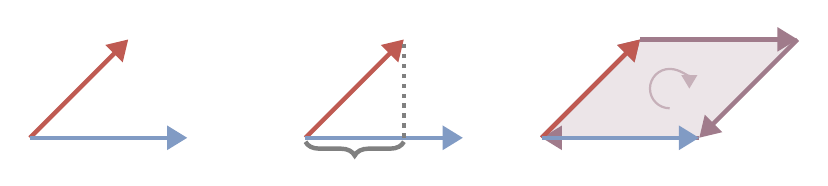
\begin{tikzpicture}[scale=0.5]

        \begin{scope}[shift={(-4,0)}]
            \coordinate (O) at (0,0);

            \def\xa{2.5}
            \def\ya{2.5}
            \coordinate (a) at (\xa,\ya);

            \def\xb{4}
            \def\yb{0}
            \coordinate (b) at (\xb,\yb);

            \draw[ultra thick, u, ->, >=Triangle] (O) -- (a);
            \draw[ultra thick, v, ->, >=Triangle] (O) -- (b);
        \end{scope}

        \begin{scope}[shift={(3,0)}]
            \coordinate (O) at (0,0);

            \def\xa{2.5}
            \def\ya{2.5}
            \coordinate (a) at (\xa,\ya);

            \def\xb{4}
            \def\yb{0}
            \coordinate (b) at (\xb,\yb);

            \draw[ultra thick, u, ->, >=Triangle] (O) -- (a);
            \draw[ultra thick, v, ->, >=Triangle] (O) -- (b);
            \draw[ultra thick, gray, dotted, overlay] (\xa,0) -- (\xa, \ya);
            \draw[decorate,gray, ultra thick,decoration={brace,amplitude=5pt,mirror}] (0,-0.1) -- (\xa, -0.1);

        \end{scope}

        \begin{scope}[shift={(9,0)}]
            \coordinate (O) at (0,0);

            \def\xa{2.5}
            \def\ya{2.5}
            \coordinate (a) at (\xa,\ya);

            \def\xb{4}
            \def\yb{0}
            \coordinate (b) at (\xb,\yb);

            \draw[ultra thick, A, ->, >=Triangle] ({\xa+\xb},{\ya}) -- (b);
            \draw[ultra thick, A, ->, >=Triangle] (a) -- ({\xa+\xb},{\ya});
            \draw[ultra thick, A, ->, >=Triangle] (b) -- (O);
            \draw[ultra thick, A, ->, >=Triangle] (O) -- (a);

            \draw[draw=none, fill=A, opacity=0.2] ({\xa+\xb},{\ya}) -- (b) -- (O) -- (a) -- cycle;
            % \node[A] at (3,1.25) {$\vec{A}$};
            \draw[A!60, thick,<-,>=Triangle] (3.75,1.25) arc[radius=0.5cm,start angle=0,delta angle=270];

            \draw[ultra thick, u, ->, >=Triangle] (O) -- (a);
            \draw[ultra thick, v, ->, >=Triangle] (O) -- (b);
        \end{scope}
        % \draw[red] (current bounding box.south west) rectangle (current bounding box.north east);
    \end{tikzpicture}

    \Huge
    \only<1>{
        $\textcolor{u}{\vec{u}} \textcolor{v}{\vec{v}} ~~~= \textcolor{u}{\vec{u}} \, \textcolor{gray}{\cdot} \, \textcolor{v}{\vec{v}} ~~+~~ \textcolor{u}{\vec{u}} \, \textcolor{A}{\wedge}\, \textcolor{v}{\vec{v}}$
    }
    \only<2-3>
    {
        $\textcolor{u}{\vec{u}} \textcolor{v}{\vec{v}} ~~~= \underbracket[0.5pt][7pt]{\textcolor{u}{\vec{u}} \, \textcolor{gray}{\cdot} \, \textcolor{v}{\vec{v}}}_\text{\huge Scalar} ~~+~~ \underbracket[0.5pt][7pt]{\textcolor{u}{\vec{u}} \, \textcolor{A}{\wedge}\, \textcolor{v}{\vec{v}}}_\text{\huge Bivector}$
    }

    \only<3>
    {
        %add space
        \vspace{1cm}
        \Huge $z ~~=~~a~~~~~+~~~~~ b \textcolor{midredgreen}{\dot{\imath}}$
    }
\end{frame}


\begin{frame}[t]{Geometric Product - vectors}

    \begin{center}

        \only<1-3>
        {
            \Huge $\textcolor{blue}{\vec{a}} \textcolor{red}{\vec{b}} = \textcolor{blue}{\vec{a}} \cdot \textcolor{red}{\vec{b}} + \textcolor{blue}{\vec{a}} \wedge \textcolor{red}{\vec{b}}$
        }


        \Large

        \only<2>
        {
            \vspace{1em}
            \begin{align*}
                \textcolor{blue}{\vec{a}}^2 & = \textcolor{blue}{\vec{a}} \cdot \textcolor{blue}{\vec{a}} + \textcolor{blue}{\vec{a}} \wedge \textcolor{blue}{\vec{a}} \\
                                            & = \textcolor{blue}{\vec{a}} \cdot \textcolor{blue}{\vec{a}}                                                              \\
                                            & = \| \textcolor{blue}{\vec{a}} \|^2
            \end{align*}
        }

        \only<3>
        {
            $\textcolor{blue}{\vec{a}}^2 = \| \textcolor{blue}{\vec{a}} \|^2$

            \vspace{1em}
            $\frac{\textcolor{blue}{\vec{a}}}{\| \textcolor{blue}{\vec{a}} \|^2} \textcolor{blue}{\vec{a}} = \frac{\| \textcolor{blue}{\vec{a}} \|^2}{\| \textcolor{blue}{\vec{a}} \|^2} = 1$

            $\textcolor{blue}{\vec{a}}^{-1} = \frac{\textcolor{blue}{\vec{a}}}{\| \textcolor{blue}{\vec{a}} \|^2}$
        }
    \end{center}
\end{frame}



\begin{frame}[t]{Geometric Product - basis vectors}

    \begin{center}

        \Large
        $\textcolor{red}{e_x} \quad \textcolor{green}{e_y} \quad \textcolor{blue}{e_z} \quad \cdots$
        \only<1>
        {
            \vspace{1em}

            $e_i^2 = \| e_i \| = 1$
            \begin{align*}
                e_i e_j & = e_i \cdot e_j + e_i \wedge e_j  \\
                        & = e_i \wedge e_j \quad (i \neq j) \\
                        & = - e_j e_i \quad (i \neq j)
            \end{align*}
        }

        \only<2>
        {
            \begin{align*}
                e_i^2   & = 1                           \\
                e_i e_j & = e_i \wedge e_j              \\
                e_i e_j & = - e_j e_i \qquad (i \neq j) \\
                e_i e_j & = e_{ij}
            \end{align*}
        }


    \end{center}
\end{frame}



\begin{frame}[t]{Geometric Product - 2d example}


    \begin{center}
        \Large
        $e_i^2 = 1; \quad e_i e_j = - e_j e_i \quad (i \neq j)$ \\
        $\vec{u}=a_1 \textcolor{red}{e_x}+ b_1 \textcolor{green}{e_y} \quad \vec{v}=a_2 \textcolor{red}{e_x}+ b_2 \textcolor{green}{e_y}$

    \end{center}

    \vspace{-2em}
    \large
    \begin{align*}
        \visible<2->{\vec{u}\vec{v}= & (a_1 \textcolor{red}{e_x}+ b_1 \textcolor{green}{e_y}) (a_2 \textcolor{red}{e_x}+ b_2 \textcolor{green}{e_y}) \\}
        \only<3>{=                   & a_1 \textcolor{red}{e_x}(a_2 \textcolor{red}{e_x}+ b_2 \textcolor{green}{e_y}) +                                                                        \\
                                     & b_1 \textcolor{green}{e_y}(a_2 \textcolor{red}{e_x}+ b_2 \textcolor{green}{e_y})\\}
        \only<4>{=                   & a_1 a_2 \textcolor{red}{e_x} \textcolor{red}{e_x} + a_1 b_2 \textcolor{red}{e_x} \textcolor{green}{e_y}                                                 \\
                                     & b_1 a_2 \textcolor{green}{e_y} \textcolor{red}{e_x} + b_1 b_2 \textcolor{green}{e_y} \textcolor{green}{e_y}\\}
        \only<5>{=                   & a_1 a_2  + a_1 b_2 \textcolor{red}{e_x} \textcolor{green}{e_y}                                                                                          \\
                                     & b_1 a_2 \textcolor{green}{e_y} \textcolor{red}{e_x} + b_1 b_2 \\}
        \only<6>{=                   & a_1 a_2  + b_1 b_2 + a_1 b_2 \textcolor{red}{e_x} \textcolor{green}{e_y} + b_1 a_2 \textcolor{green}{e_y} \textcolor{red}{e_x}\\}
        \only<7>{=                   & a_1 a_2  + b_1 b_2 + a_1 b_2 \textcolor{red}{e_x} \textcolor{green}{e_y} - b_1 a_2 \textcolor{red}{e_x} \textcolor{green}{e_y}\\}
        \only<8>{=                   & a_1 a_2  + b_1 b_2 + (a_1 b_2 - b_1 a_2) \textcolor{red}{e_x} \textcolor{green}{e_y}\\}
        \only<9>{=                   & a_1 a_2  + b_1 b_2 + (a_1 b_2 - b_1 a_2) \textcolor{midredgreen}{e_{xy}}\\}
        \only<10->{=                 & a_1 a_2  + b_1 b_2 + (a_1 b_2 - b_1 a_2) \textcolor{mixAll}{\mathbf{I}}_2\\}
    \end{align*}
\end{frame}



\begin{frame}{2d pseudoscalar}
    \centering
    \Large
    \only<1-7>{$(\textcolor{mixAll}{\mathbf{I}}_2)^2$}
    \only<2-5>{$=(\textcolor{midredgreen}{e_{xy}})^2$}
    \only<3>{$=\textcolor{red}{e_x} \textcolor{green}{e_y} \textcolor{red}{e_x} \textcolor{green}{e_y}$}
    \only<4>{$=-\textcolor{red}{e_x} \textcolor{green}{e_y} \textcolor{green}{e_y} \textcolor{red}{e_x}$}
    \only<5>{$=-\textcolor{red}{e_x} \textcolor{red}{e_x}$}
    \only<6-7>{$=-1$}
    \only<7>{$=\textcolor{mixAll}{\dot{\imath}}^2$}
    \only<8->{$\textcolor{mixAll}{\mathbf{I}}_2 \equiv \textcolor{mixAll}{\dot{\imath}}$}

    \only<9->{
        $\vec{u}\vec{v} = a_1 a_2  + b_1 b_2 + (a_1 b_2 - b_1 a_2) \textcolor{mixAll}{\dot{\imath}}$
    }

    \vspace{2em}

    \only<10->{
        $\vec{u}\vec{v}$ is a complex number!
    }

    \visible<11>{
        \renewcommand\arraystretch{1.0}
        ~\\~\\
        \textbf{Complex Numbers are naturally included in 2d GA!}
    }
\end{frame}



\begin{frame}[t]{Geometric Product - 3d example}


    \begin{center}
        \Large
        $e_i^2 = 1; \quad e_i e_j = - e_j e_i \quad (i \neq j)$ \\
        $\vec{u}=a_1 \textcolor{red}{e_x}+ b_1 \textcolor{green}{e_y}+ c_1 \textcolor{blue}{e_z} \quad \vec{v}=a_2 \textcolor{red}{e_x}+ b_2 \textcolor{green}{e_y}+ c_2 \textcolor{blue}{e_z}$

    \end{center}

    \vspace{-2em}
    \large
    \begin{align*}
        \visible<2->{\vec{u}\vec{v}= & (a_1 \textcolor{red}{e_x}+ b_1 \textcolor{green}{e_y}+ c_1 \textcolor{blue}{e_z}) (a_2 \textcolor{red}{e_x}+ b_2 \textcolor{green}{e_y}+ c_2 \textcolor{blue}{e_z}) \\}
        \only<3>{=                   & a_1 \textcolor{red}{e_x}(a_2 \textcolor{red}{e_x}+ b_2 \textcolor{green}{e_y}+ c_2 \textcolor{blue}{e_z}) +                                                                                   \\
                                     & b_1 \textcolor{green}{e_y}(a_2 \textcolor{red}{e_x}+ b_2 \textcolor{green}{e_y}+ c_2 \textcolor{blue}{e_z}) +                                                                                 \\
                                     & c_1 \textcolor{blue}{e_z}(a_2 \textcolor{red}{e_x}+ b_2 \textcolor{green}{e_y}+ c_2 \textcolor{blue}{e_z}) \\}
        \only<4>{=                   & a_1 a_2 \textcolor{red}{e_x} \textcolor{red}{e_x} + a_1 b_2 \textcolor{red}{e_x} \textcolor{green}{e_y} + a_1 c_2 \textcolor{red}{e_x} \textcolor{blue}{e_z} +                                \\
                                     & b_1 a_2 \textcolor{green}{e_y} \textcolor{red}{e_x} + b_1 b_2 \textcolor{green}{e_y} \textcolor{green}{e_y} + b_1 c_2 \textcolor{green}{e_y} \textcolor{blue}{e_z} +                          \\
                                     & c_1 a_2 \textcolor{blue}{e_z} \textcolor{red}{e_x} + c_1 b_2 \textcolor{blue}{e_z} \textcolor{green}{e_y} + c_1 c_2 \textcolor{blue}{e_z} \textcolor{blue}{e_z}\\}
        \only<5>{=                   & a_1 a_2  + a_1 b_2 \textcolor{red}{e_x} \textcolor{green}{e_y} + a_1 c_2 \textcolor{red}{e_x} \textcolor{blue}{e_z} +                                                                         \\
                                     & b_1 a_2 \textcolor{green}{e_y} \textcolor{red}{e_x} + b_1 b_2  + b_1 c_2 \textcolor{green}{e_y} \textcolor{blue}{e_z} +                                                                       \\
                                     & c_1 a_2 \textcolor{blue}{e_z} \textcolor{red}{e_x} + c_1 b_2 \textcolor{blue}{e_z} \textcolor{green}{e_y} + c_1 c_2 \\}
        \only<6>{=                   & a_1 a_2  + b_1 b_2 + c_1 c_2 +                                                                                                                                                                \\
                                     & a_1 b_2 \textcolor{red}{e_x} \textcolor{green}{e_y} + b_1 a_2 \textcolor{green}{e_y} \textcolor{red}{e_x} +                                                                                   \\
                                     & a_1 c_2 \textcolor{red}{e_x} \textcolor{blue}{e_z} + c_1 a_2 \textcolor{blue}{e_z} \textcolor{red}{e_x} +                                                                                     \\
                                     & b_1 c_2 \textcolor{green}{e_y} \textcolor{blue}{e_z} + c_1 b_2 \textcolor{blue}{e_z} \textcolor{green}{e_y} \\}
        \only<7>{=                   & a_1 a_2  + b_1 b_2 + c_1 c_2 +                                                                                                                                                                \\
                                     & a_1 b_2 \textcolor{red}{e_x} \textcolor{green}{e_y} - b_1 a_2 \textcolor{red}{e_x} \textcolor{green}{e_y} +                                                                                   \\
                                     & a_1 c_2 \textcolor{red}{e_x} \textcolor{blue}{e_z} - c_1 a_2 \textcolor{red}{e_x} \textcolor{blue}{e_z} +                                                                                     \\
                                     & b_1 c_2 \textcolor{green}{e_y} \textcolor{blue}{e_z} - c_1 b_2 \textcolor{green}{e_y} \textcolor{blue}{e_z} \\}
        \only<8>{=                   & a_1 a_2  + b_1 b_2 + c_1 c_2 +                                                                                                                                                                \\
                                     & (a_1 b_2 - b_1 a_2) \textcolor{red}{e_x} \textcolor{green}{e_y} +                                                                                                                             \\
                                     & (a_1 c_2 - c_1 a_2) \textcolor{red}{e_x} \textcolor{blue}{e_z} +                                                                                                                              \\
                                     & (b_1 c_2 - c_1 b_2) \textcolor{green}{e_y} \textcolor{blue}{e_z} \\}
        \only<9>{=                   & a_1 a_2  + b_1 b_2 + c_1 c_2 +                                                                                                                                                                \\
                                     & (a_1 b_2 - b_1 a_2) \textcolor{midredgreen}{e_{xy}} +                                                                                                                                         \\
                                     & (a_1 c_2 - c_1 a_2) \textcolor{midredblue}{e_{xz}} +                                                                                                                                          \\
                                     & (b_1 c_2 - c_1 b_2) \textcolor{midgreenblue}{e_{yz}} \\}
        \only<10>{=                  & a_1 a_2  + b_1 b_2 + c_1 c_2 + (a_1 b_2 - b_1 a_2) \textcolor{midredgreen}{e_{xy}} +                                                                                                          \\
                                     & ~~~~~~~~~~~~~~~~~~~~~~~~~~~(a_1 c_2 - c_1 a_2) \textcolor{midredblue}{e_{xz}} +                                                                                                               \\
                                     & ~~~~~~~~~~~~~~~~~~~~~~~~~~~(b_1 c_2 - c_1 b_2) \textcolor{midgreenblue}{e_{yz}} \\}
    \end{align*}
\end{frame}


%%%%%%%%%%%%%%%%%%
\begin{frame}[t]{3d bivectors}
    \centering
    \Large
    \textbf{If we rename}
    $$
        \textcolor{midgreenblue}{i} \equiv -\textcolor{midgreenblue}{e_{yz}}~~~~~
        \textcolor{midredblue}{j} \equiv \textcolor{midredblue}{e_{xz}}~~~~~
        \textcolor{midredgreen}{k} \equiv -\textcolor{midredgreen}{e_{xy}}
    $$

    \only<2-3>{
        \textbf{then}
        \renewcommand\arraystretch{1.5}
        $$
            \left.
            \begin{array}{r}
                \textcolor{midgreenblue}{i}^2  = \textcolor{midredblue}{j}^2 = \textcolor{midredgreen}{k}^2 = -1 \\
                \textcolor{midgreenblue}{i}\textcolor{midredblue}{j}=\textcolor{midredgreen}{k} ~~~~
                \textcolor{midredblue}{j}\textcolor{midredgreen}{k}=\textcolor{midgreenblue}{i} ~~~~
                \textcolor{midredgreen}{k}\textcolor{midgreenblue}{i}=\textcolor{midredblue}{j}                  \\
                \textcolor{midredblue}{j}\textcolor{midgreenblue}{i}=-\textcolor{midgreenblue}{i}\textcolor{midredblue}{j} ~~~~
                \textcolor{midredgreen}{k}\textcolor{midredblue}{j}=-\textcolor{midredblue}{j}\textcolor{midredgreen}{k} ~~~~
                \textcolor{midgreenblue}{i}\textcolor{midredgreen}{k}=-\textcolor{midredgreen}{k}\textcolor{midgreenblue}{i}
            \end{array}
            \right\rbrace
            \only<3>
            {
                \text{Hamilton's algebra}
            }
        $$
    }
    \only<4-5>
    {
        \begin{align*}
            \vec{u}\vec{v} & = a_1 a_2  + b_1 b_2 + c_1 c_2+(c_1 b_2 - b_1 c_2) \textcolor{midgreenblue}{\dot{\imath}}+ \\
                           & ~~~~~~~~~~~~~~~~~~~~~~~~~~~~~~~(a_1 c_2 - c_1 a_2) \textcolor{midredblue}{\dot{\jmath}} +  \\
                           & ~~~~~~~~~~~~~~~~~~~~~~~~~~~~~~~(b_1 a_2 - a_1 b_2) \textcolor{midredgreen}{k}              \\
        \end{align*}

        \textbf{Quaternions are naturally included in 3d Geometric Algebra!}
    }
\end{frame}


\section{Transformations}

\begin{frame}{Reflection}
\end{frame}


\begin{frame}{What about 2 reflexions?}
    \hfill\href{https://enkimute.github.io/ganja.js/examples/coffeeshop.html\#yYimFv544&fullscreen}{\beamergotobutton{2D rotation}}
\end{frame}


\begin{frame}{Rotation}
    ... and what if reflecting lines are parallel? \\
    \hfill\href{https://enkimute.github.io/ganja.js/examples/coffeeshop.html\#yYimFv544&fullscreen}{\beamergotobutton{2D rotation}}
\end{frame}


\begin{frame}{Translation}
    \begin{center}
        \only<1>{%
            \begin{tikzpicture}
                % planes
                \draw (0,-1) node[below]{$\mathbf{b}$} -- (0,1) ;
                \draw (2,-1) node[below]{$\mathbf{a}$} -- (2,1) ;
                % intial points
                \draw[blue,fill=blue] (-0.5,0.5) circle (0.05);
                \draw[red,fill=red]  (-3,-0.5) circle (0.05);
                % clip
                \clip (-4,1) rectangle (4,1);
            \end{tikzpicture}
        }%
        \only<2>{%
            \begin{tikzpicture}
                % planes
                \draw (0,-1) node[below]{$\mathbf{b}$} -- (0,1) ;
                \draw (2,-1) node[below]{$\mathbf{a}$} -- (2,1) ;
                % intial points
                \draw[blue,fill=blue] (-0.5,0.5) circle (0.05);
                \draw[red,fill=red]  (-3,-0.5) circle (0.05);
                % first reflexion
                \draw[blue,fill=blue] (0.5,0.5) circle (0.05);
                \draw[red,fill=red]  (3,-0.5) circle (0.05);
                % line
                \path[gray,->,>=latex] (-0.5,0.5) edge[out=20,in=160] (0.5,0.5);
                \path[gray,->,>=latex] (-3,-0.5)  edge[out=10,in=170] (3,-0.5);
                % clip
                \clip (-4,1) rectangle (4,1);
            \end{tikzpicture}
        }%
        \only<3>{%
            \begin{tikzpicture}
                % planes
                \draw (0,-1) node[below]{$\mathbf{b}$} -- (0,1) ;
                \draw (2,-1) node[below]{$\mathbf{a}$} -- (2,1) ;
                % intial points
                \draw[blue,fill=blue] (-0.5,0.5) circle (0.05);
                \draw[red,fill=red]  (-3,-0.5) circle (0.05);
                % first reflexion
                \draw[gray,fill=gray] (0.5,0.5) circle (0.05);
                \draw[gray,fill=gray]  (3,-0.5) circle (0.05);
                % second reflexion
                \draw[blue,fill=blue] (3.5,0.5) circle (0.05);
                \draw[red,fill=red]  (1,-0.5) circle (0.05);
                % line
                \path[gray,->,>=latex] (0.5,0.5) edge[out=20,in=160] (3.5,0.5);
                \path[gray,->,>=latex] (3,-0.5)  edge[out=170,in=10] (1,-0.5);
                % clip
                \clip (-4,1) rectangle (4,1);
            \end{tikzpicture}
        }%
        \only<4>{%
            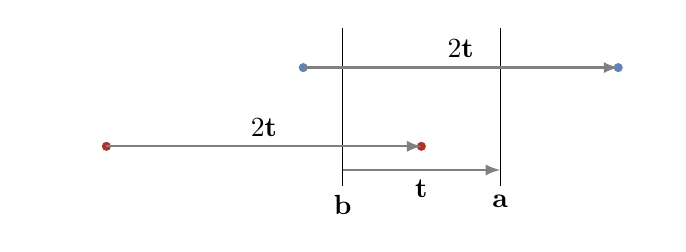
\begin{tikzpicture}
                % planes
                \draw (0,-1) node[below]{$\mathbf{b}$} -- (0,1) ;
                \draw (2,-1) node[below]{$\mathbf{a}$} -- (2,1) ;
                % intial points
                \draw[blue,fill=blue] (-0.5,0.5) circle (0.05);
                \draw[red,fill=red]  (-3,-0.5) circle (0.05);
                % second reflexion
                \draw[blue,fill=blue] (3.5,0.5) circle (0.05);
                \draw[red,fill=red]  (1,-0.5) circle (0.05);
                % line
                \draw[gray,thick,->,>=latex] (-0.5,0.5) -- node[midway,above,black]{$2\mathbf{t}$} (3.5,0.5);
                \draw[gray,thick,->,>=latex] (-3,-0.5)  -- node[midway,above,black]{$2\mathbf{t}$} (1,-0.5);
                %translation
                \draw[gray,thick,->,>=latex] (0,-0.8) -- node[midway,below,black]{$\mathbf{t}$} (2,-0.8);
                % clip
                \clip (-4,1) rectangle (4,1);
            \end{tikzpicture}
        }%
        \only<5>{%
            \begin{tikzpicture}
                % planes
                \draw[white] (0,-1) node[below]{$\mathbf{b}$} -- (0,1) ;
                \draw[white] (2,-1) node[below]{$\mathbf{a}$} -- (2,1) ;
                % intial points
                \draw[blue,fill=blue] (-0.5,0.5) circle (0.05);
                \draw[red,fill=red]  (-3,-0.5) circle (0.05);
                % second reflexion
                \draw[blue,fill=blue] (3.5,0.5) circle (0.05);
                \draw[red,fill=red]  (1,-0.5) circle (0.05);
                % line
                0\draw[gray,thick,->,>=latex] (-0.5,0.5) -- node[midway,above,black]{$2\mathbf{t}$} (3.5,0.5);
                \draw[gray,thick,->,>=latex] (-3,-0.5)  -- node[midway,above,black]{$2\mathbf{t}$} (1,-0.5);
                % clip
                \clip (-4,1) rectangle (4,1);
            \end{tikzpicture}
        }%
    \end{center}
    %\textbf{Double reflection:}
    %\begin{itemize}
    %\item $\mathbf{T}=\mathbf{ab} = 1 + \displaystyle\frac{t}{2}\mathbf{P}$
    %\item $\mathbf{X}'=\mathbf{ab} \mathbf{X} (\mathbf{ab})^{-1} = \mathbf{T} \mathbf{X} \mathbf{\widetilde{T}}$
    %\item $\mathbf{P} \rightarrow$ point at infinity $\Rightarrow \mathbf{P}^2=0$ 
    %\end{itemize}
\end{frame}



\begin{frame}{But in 3D?}
\end{frame}


%%%%%%%%%%%%%%%%%%%
\begin{frame}{Interpretation}
    \begin{center}
        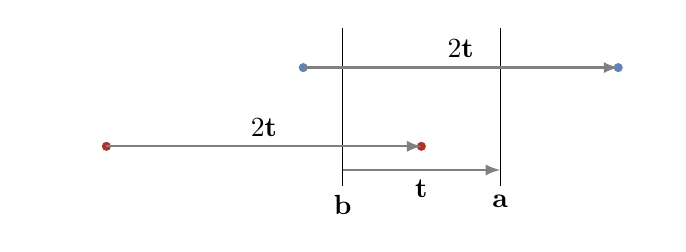
\begin{tikzpicture}
            % planes
            \draw (0,-1) node[below]{$\mathbf{b}$} -- (0,1) ;
            \draw (2,-1) node[below]{$\mathbf{a}$} -- (2,1) ;
            % intial points
            \draw[blue,fill=blue] (-0.5,0.5) circle (0.05);
            \draw[red,fill=red]  (-3,-0.5) circle (0.05);
            % second reflexion
            \draw[blue,fill=blue] (3.5,0.5) circle (0.05);
            \draw[red,fill=red]  (1,-0.5) circle (0.05);
            % line
            \draw[gray,thick,->,>=latex] (-0.5,0.5) -- node[midway,above,black]{$2\mathbf{t}$} (3.5,0.5);
            \draw[gray,thick,->,>=latex] (-3,-0.5)  -- node[midway,above,black]{$2\mathbf{t}$} (1,-0.5);
            %translation
            \draw[gray,thick,->,>=latex] (0,-0.8) -- node[midway,below,black]{$\mathbf{t}$} (2,-0.8);
            % clip
            \clip (-4,1) rectangle (4,1);
        \end{tikzpicture}
    \end{center}
    \begin{itemize}
        \item any combinaison of 2 successive reflexions $\leftrightarrow$ combinaison of rotation / translation \\
              $\hookrightarrow$ rigid transformation
        \item quaternions and dual quaternions are a special form of motors, in 3D.
        \item motors (double reflexion) works in any dimension !
    \end{itemize}
\end{frame}



%%%%%%%%%%%%%%%%%%
\begin{frame}{Reflexions are generic}
    $$ \mathbf{a}\Big( \textcolor{blue}{\mathbf{x} \wedge \mathbf{y} \wedge  ... \wedge \mathbf{z}} \Big) \mathbf{a}^{-1}
        = (\mathbf{a}\textcolor{blue}{\mathbf{x}} \mathbf{a}^{-1}) \wedge (\mathbf{a}\textcolor{blue}{\mathbf{y}} \mathbf{a}^{-1}) \wedge  ... \wedge  (\mathbf{a}\textcolor{blue}{\mathbf{z}} \mathbf{a}^{-1})$$
    ~\\
    \textbf{Same versor for any object:}
    $$
        \mathbf{a}
        \left\lbrace
        \begin{array}{c}
            \text{point} \\
            \text{line}  \\
            \text{plane} \\
            \vdots
        \end{array}
        \right\rbrace
        \mathbf{a}^{-1}
    $$
\end{frame}






%%%%%%%%%%%%%%%%%%%%%%%%%%%%%%%%%%%%%%%%%%%%%%%%%%%%%%%%%%%%%%%%%%%%%%%
\section{Demo}

%%%%%%%%%%%%%%%%
\begin{frame}{Demo in Python}
    \hfill\href{https://tbuli.github.io/teahouse/lab/index.html}{\beamergotobutton{a cube and a string}}
\end{frame}


\begin{frame}{Geometric algebra}
    conclusion
\end{frame}



\end{document}


